\documentclass{article}

\usepackage{graphicx}
\usepackage{tikz}
\usepackage{tikzsymbols}
\usetikzlibrary{calc,patterns,shapes.geometric}
\pagestyle{empty}
\usepackage[margin=0pt]{geometry}
\geometry{papersize={14in,12in}}

\def\centerarc[#1](#2)(#3:#4:#5){\draw[#1] ($(#2)+({#5*cos(#3)},{#5*sin(#3)})$) arc (#3:#4:#5);}

\begin{document}
	\begin{figure}
		\centering
		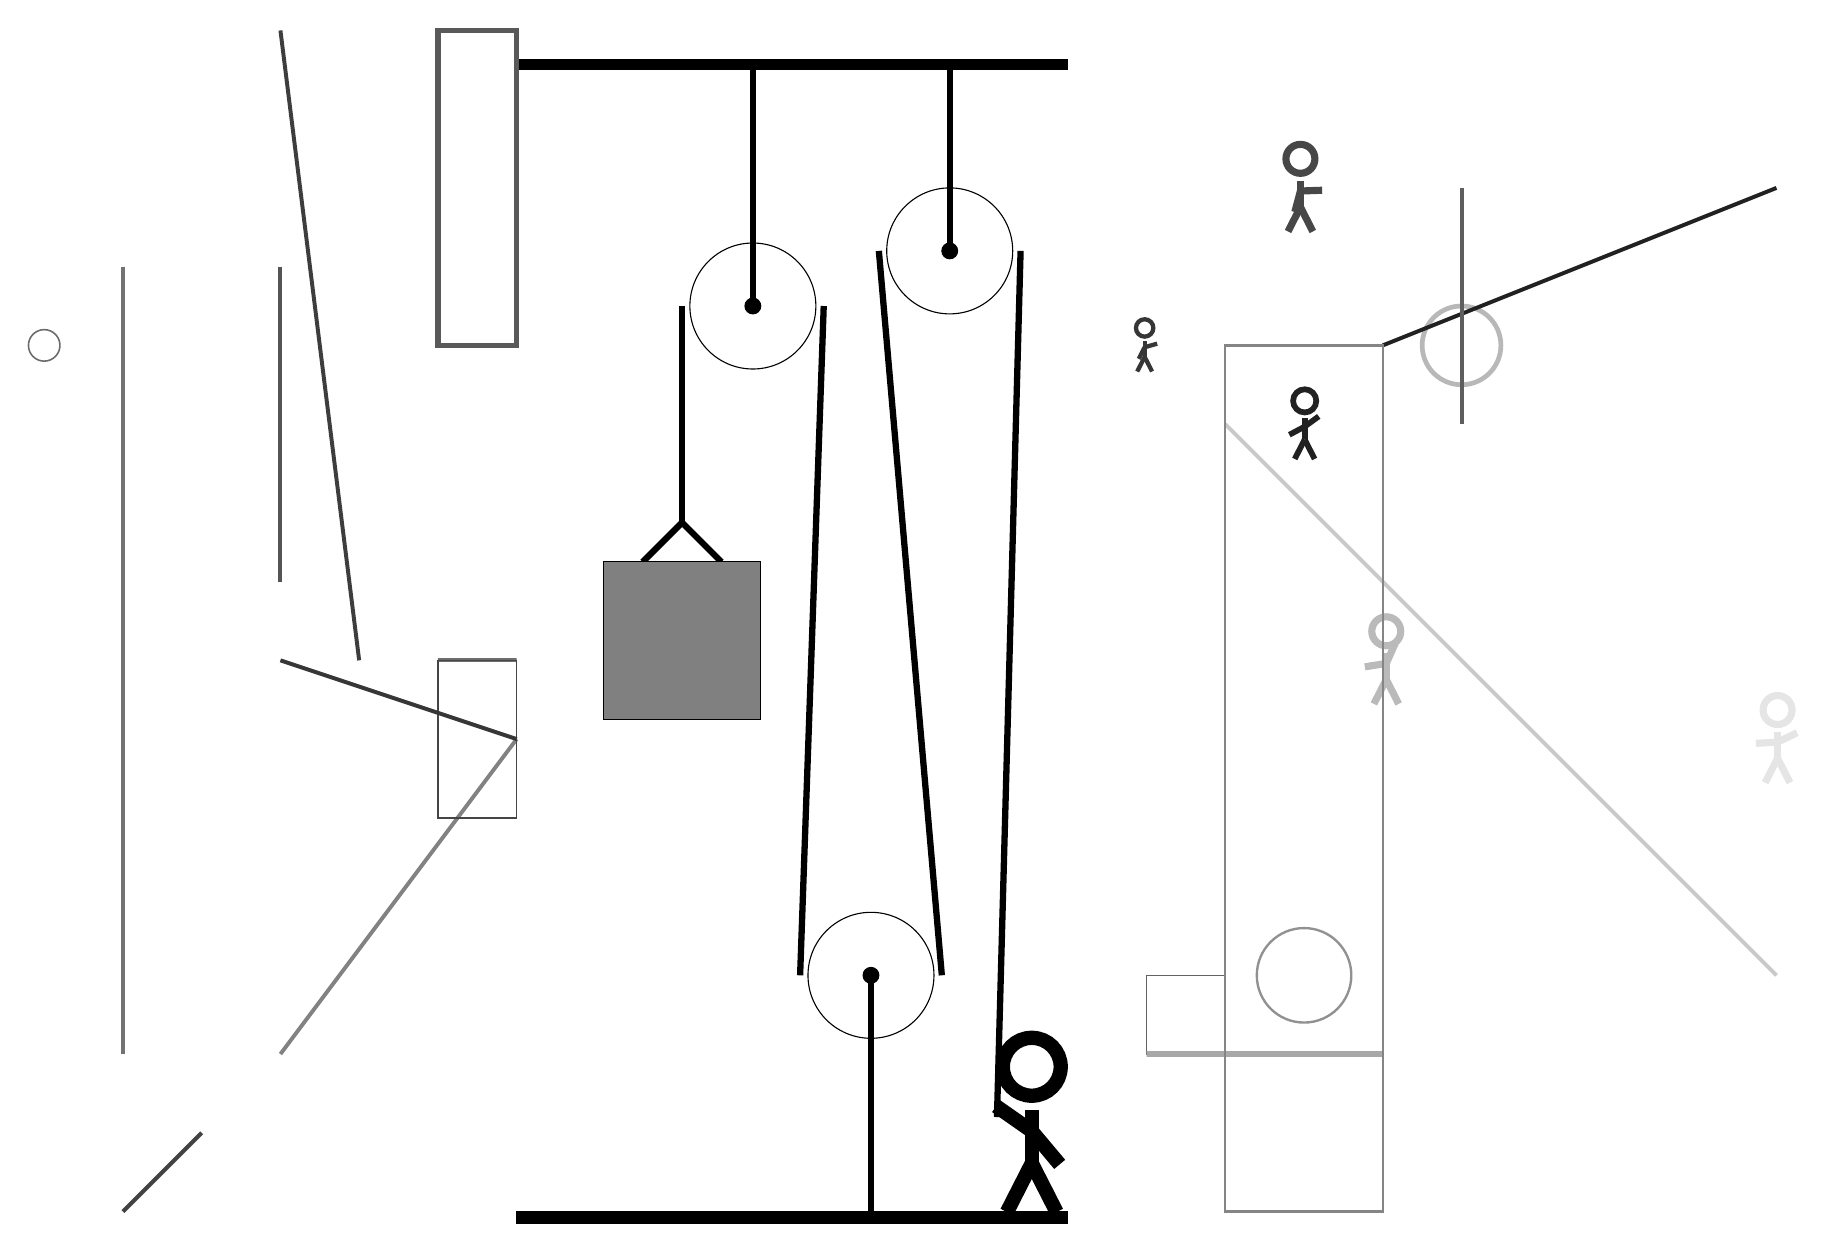
\begin{tikzpicture}
			%%%%% START %%%%%
			
			\draw[fill=black] (-2, 11.5) rectangle (5, 11.625);
			
			\draw (1, 8.5) circle (0.8);
			\draw[fill=black] (1, 8.5) circle (0.1);
			\draw[line width=0.8mm]  (1, 11.5) -- (1, 8.5);
			
			\draw[fill=white](2.5, 0.0) circle (0.8);
			\draw[fill=black] (2.5, 0.0) circle (0.1);
			\draw[line width=0.8mm]  (2.5, -3) -- (2.5, 0.0);
			
			\draw[fill=white](3.5, 9.2) circle (0.8);
			\draw[fill=black] (3.5, 9.2) circle (0.1);
			\draw[line width=0.8mm] (3.5, 11.5) -- (3.5, 9.2);
			
			\draw[line width=0.5mm, color=black!49](-5, -1) -- (-2, 3);
			
			\draw[line width=0.5mm, color=black!76](-4, 4) -- (-5, 12);
			\draw[line width=0.5mm, color=black!57] (-2, 4) rectangle (-3, 4);
			\node[line width=0.3mm, color=black!27] at (9, 4) {\Strichmaxerl[5][9][66]};
			
			\draw [line width=0.3mm, color=black!43](8, 0) circle (0.6);
			\node[line width=0.3mm, color=black!87] at (8, 7) {\Strichmaxerl[4][28][36]};
			
			\node[line width=0.6mm, color=black!79] at (6, 8) {\Strichmaxerl[3][63][16]};
			
			\draw [line width=0.6mm, color=black!28](10, 8) circle (0.5);
			\draw[line width=0.5mm, color=black!87](9, 8) -- (14, 10);
			\draw [line width=0.2mm, color=black!58](-8, 8) circle (0.2);
			
			\node[line width=0.5mm, color=black!10] at (14, 3) {\Strichmaxerl[5][3][26]};
			\node[line width=0.3mm, color=black!72] at (8, 10) {\Strichmaxerl[5][75][2]};
			\draw[line width=0.7mm, color=black!65] (-2, 8) rectangle (-3, 12);
			
			\draw[line width=0.2mm, color=black!61] (7, 0) rectangle (6, -1);
			\draw[line width=0.5mm, color=black!74](-7, -3) -- (-6, -2);
			\draw[line width=0.5mm, color=black!67](-5, 5) -- (-5, 9);
			
			\draw[line width=0.5mm, color=black!21](7, 7) -- (14, 0);
			
			\draw[line width=0.5mm, color=black!63](10, 7) -- (10, 10);
			\draw[line width=0.5mm, color=black!55](-7, 9) -- (-7, -1);
			
			\draw[line width=0.2mm, color=black!73] (-3, 4) rectangle (-2, 2);
			\draw[line width=0.5mm, color=black!79](-5, 4) -- (-2, 3);
			
			\draw[line width=0.7mm, color=black!34] (6, -1) rectangle (9, -1);
			\draw[line width=0.3mm, color=black!48] (7, 8) rectangle (9, -3);
			
			\draw[line width=0.8mm] (-0.4, 5.25) -- (0.1, 5.75) -- (0.6, 5.25);
			\draw[fill=black!50] (-0.9, 5.25) rectangle (1.1, 3.25);
			
			\draw[line width=0.8mm] (0.1, 8.5) -- (0.1, 5.75);
			\centerarc[line width=0.8mm](1, 8.5)(0:180:0.9);
			\draw[line width=0.8mm](1.9, 8.5) -- (1.6, 0.0);
			\centerarc[line width=0.8mm](2.5, 0.0)(180:360:0.9);
			\draw[line width=0.8mm](3.4, 0.0) -- (2.6, 9.2);
			\centerarc[line width=0.8mm](3.5, 9.2)(0:180:0.9);
			\draw[line width=0.8mm](4.4, 9.2) -- (4.1, -1.8);
			
			\node at (4.5, -1.9) {\Strichmaxerl[10][-35][-50]};
			
			\draw[fill=black] (-2, -3) rectangle (5, -3.15);
			
			%%%%% END %%%%%
		\end{tikzpicture}
	\end{figure}	
\end{document}